\documentclass{article}
\usepackage{tikz}
\usepackage{pgf}
\usepackage{ifthen}

\begin{document}

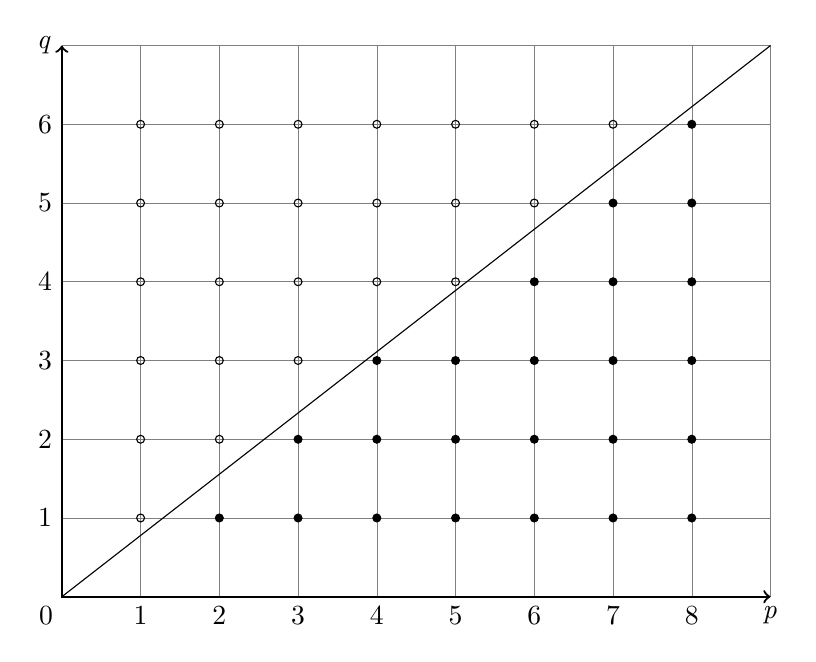
\begin{tikzpicture}
    % p = 17, q = 13
    \draw[help lines, step = 1] (0,0) grid (9,7);   % 画辅格子
    \draw [thick, <->] (0,7) -- (0,0) -- (9,0);     % 坐标轴
    \node[below] at (-0.2,0){0};                    % 坐标 0
    \node[below] at (9,0){\emph{p}};                % 坐标轴标注 p
    \node[left] at (0,7){\emph{q}};                 % 坐标轴标注 q
    % 画刻度
    \foreach \x in {1,2,...,8}
    {
        \node[below] at(\x,0){\x};
    }
    \foreach \y in {1,2,...,6}
    {
        \node[left] at(0,\y){\y};
    }

    % 画点
    \foreach \x in {1,2,...,8}
    {
        \foreach \y in {1,2,...,6}
        {
            \pgfmathparse{(13 / 17) * \x + 1}       % 计算 y 的上界,+1 是为了避免取整导致下面判断
            \ifthenelse{\y < \pgfmathresult}
            {
                \draw[fill] (\x,\y) circle [radius=0.05];
            }
            {
                \draw (\x,\y) circle [radius=0.05];
            }
        }
    }
    % 画线
    \draw (0,0) -- (9,7);

\end{tikzpicture}

\end{document}